% !TEX root = thesis.tex
\FloatBarrier
\section{Results}
\label{sec:results}



%\subsection{Data}
%\begin{figure}[htp]
%\centering
%%\begin{subfigure}{0.95\textwidth}
%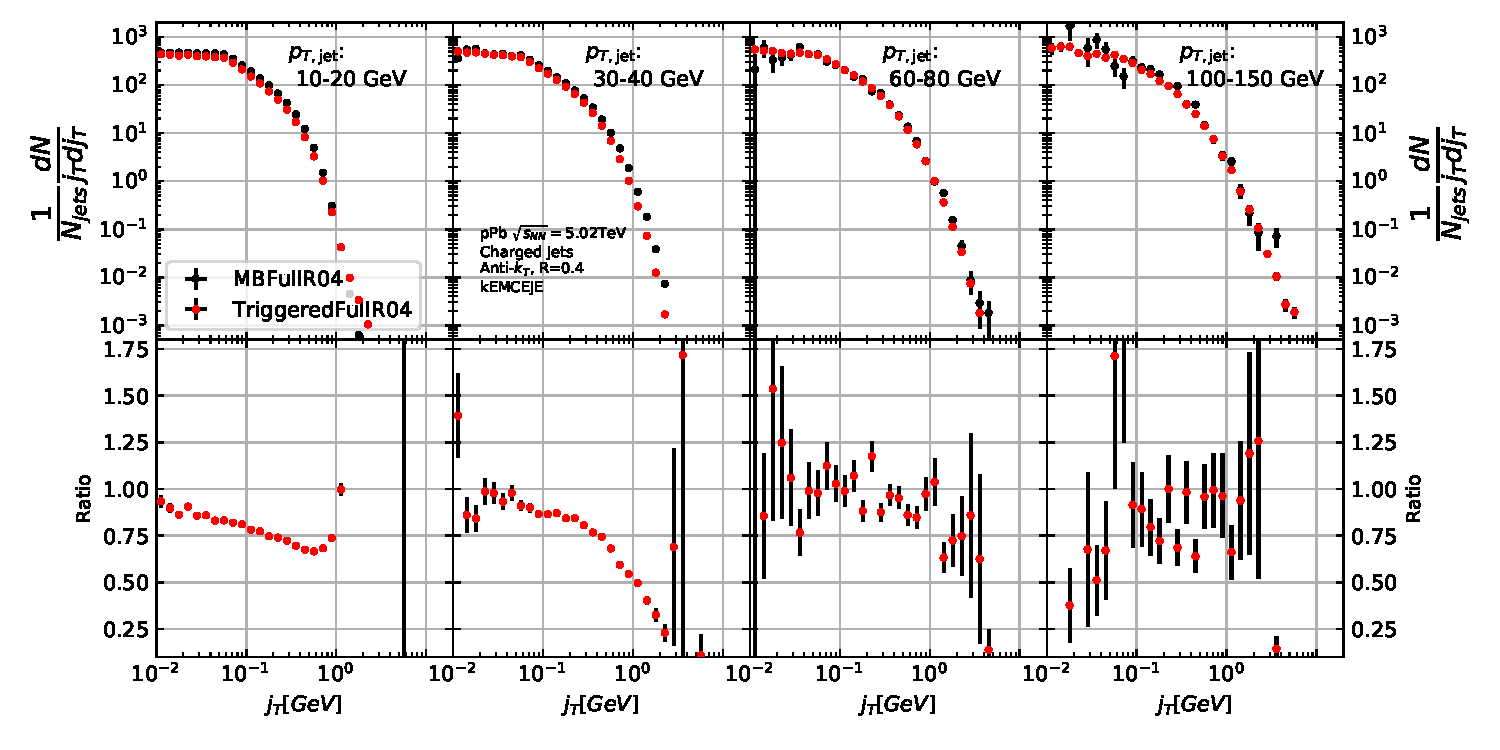
\includegraphics[width=0.95\textwidth]{results/MBvsTriggeredFullJetsR04JetConeJt.pdf} 
%%Tag 20170810 python2.7 Python/MBtoTriggeredComparison.py legotrain_CF_pPb-1053_20170223-2002_LHC13bcde.root
%
%%\includegraphics[width=0.95\textwidth]{results/OverlayjetjtIncl_T02_\figComment}
%\caption{Comparison between minimum bias and triggered datasets }
%%\end{subfigure}
%%\begin{subfigure}{0.5\textwidth}
%%%\includegraphics[width=0.95\textwidth]{results/OverlayjetjtIncl_T06_\figComment}
%%%\caption{Jet $\pt{}$ 80-100 GeV}
%%\end{subfigure}
%\end{figure}
%\subsection{Inclusive results}


%As outlined in Section ~\ref{sec:analysis} the inclusive $\jt{}$ distributions and corresponding backgrounds are obtained for different jet $\pt{}$ bins starting from $10\:\gev < \pt{jet} < 20\:\gev$. Later the lowest $\pt{}$ bins are omitted because of problems in unfolding and fitting. The results are shown in Fig.~\ref{fig:inclusive}. The background distribution the figure is obtained by the perpendicular cone method.







%\subsection{$\jt{} signal distributions$}
In this section I present the final results for $\jt{}$ signals. After unfolding and subtracting the background contribution we get the final $\jt{}$ distributions. These are then fitted using the two component model. Figure~\ref{fig:fits} shows $\jt{}$ distributions for two different $\pt{jet}$ bins with $\unit[60]{\gev}< \pt{jet}  < \unit[80]{\gev}$ and $\unit[100]{\gev}< \pt{jet}  < \unit[150]{\gev}$. Additional $\pt{jet}$ bins are shown in appendix \ref{app:a}. It is clear that the distributions get wider with increasing $\pt{jet}$. In part this is explained by kinematics; In a jet cone the cone size sets limits on the possible $\jt{}$ values. For a given $\pt{,track}$ the maximum $\jt{}$ value is approximately

\begin{equation}
\jt{max} \approx R\cdot \pt{,track},
\end{equation}

\noindent using the small angle approximation. This illustrated in Fig.~\ref{fig:jtmax}
\begin{figure}[h!]
\tikzset{
photon/.style={decorate, decoration={snake}, draw=red},
particlearrow/.style={draw=blue, postaction={decorate},
    decoration={markings,mark=at position .5 with {\arrow[draw=black]{>}}}},
antiparticlearrow/.style={draw=blue, postaction={decorate},
    decoration={markings,mark=at position .5 with {\arrow[draw=black]{>}}}},
particle/.style={draw=blue},
antiparticle/.style={draw=blue},
gluon/.style={decorate, draw=orange,
    decoration={coil,amplitude=4pt, segment length=5pt}}
 }
\centering
\begin{tikzpicture}[scale= 3]
\coordinate[] (a);
\coordinate[above right = 1.2cm and 3cm of a,label=right:{\color{black!60}Jet Cone}] (b);
\coordinate[below right = 1.2cm and 3cm of a] (c);
\coordinate[above right = 0.8cm and 2cm  of a] (d);
\coordinate[right = 2cm of a] (e);
\coordinate[right = 4cm of a] (g);
\coordinate[right = 3cm of a] (f);
\draw[thick, black!60] (a) -- (b);
\draw[thick, black!60] (a) -- (c); 
\draw[thick, blue,->] (a) -- node[label=above:$\vec{p}_\mathrm{track}$] {}  (d);
\draw[thick, black!40, ->] (a) -- (g);
\draw[dashed,blue,->] (e) -- node[label=right:$\jt{max}$] {}  (d);
\draw[thick, black!60, ->] (f) --  node[label=right:$R$] {}  (c);
\end{tikzpicture}
\caption{\jt{} has maximum value defined by the cone size and track momentum $\vec{p}_\mathrm{track}$}
\label{fig:jtmax}
\end{figure}



We fit the distribution using the two component fit function presented in Sec.~\ref{sec:fitting}. These are also shown in Fig.~\ref{fig:fits}. Aside from statistical fluctuations the fits describe the data well. It should be noted that fitting a Gaussian alone would produce the same result as the Gaussian component in the combined fit function.


\begin{figure}[htb]
\centering
\begin{subfigure}{0.44\textwidth}
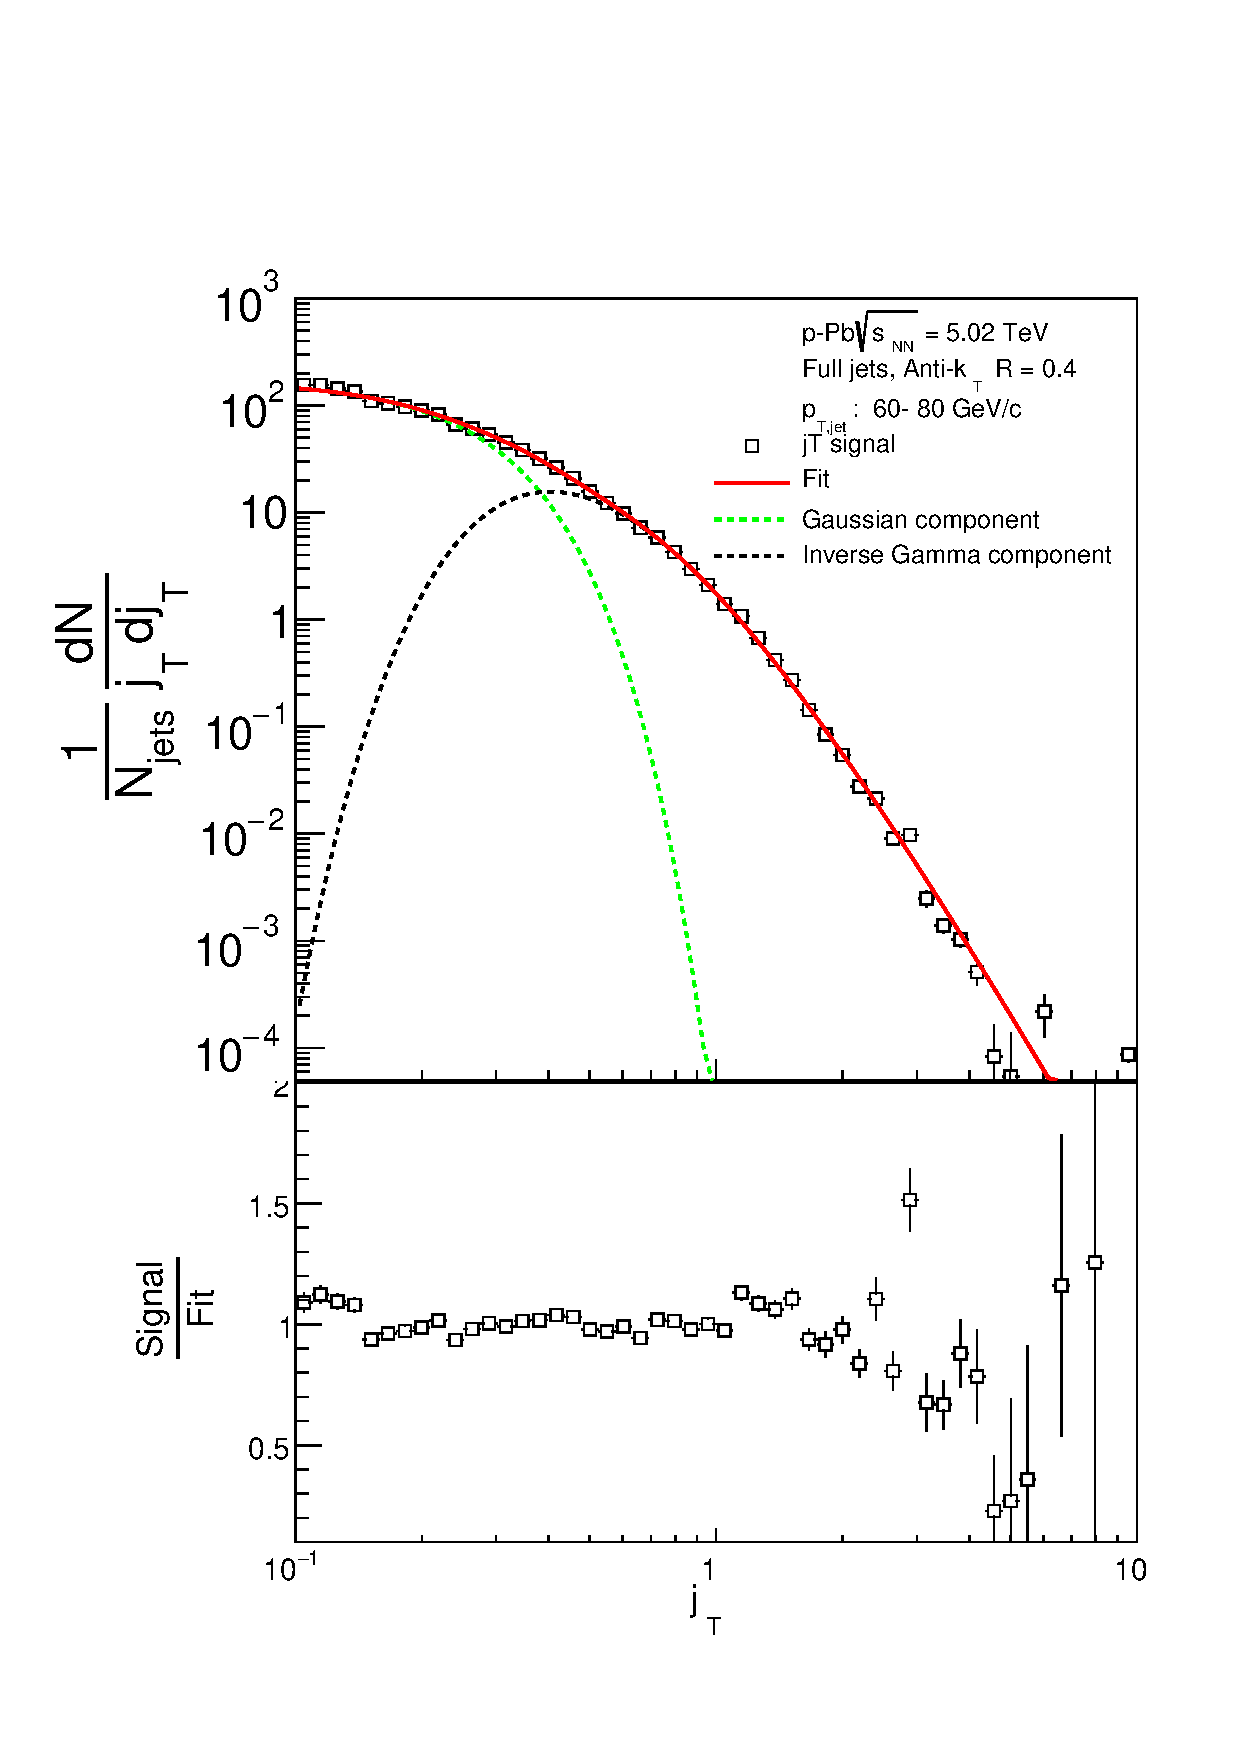
\includegraphics[width=0.95\textwidth]{results/JetConejTSignalFit/JetConejTSignalFitNFin00JetPt05perconeBgBayes}
\end{subfigure}
\begin{subfigure}{0.44\textwidth}
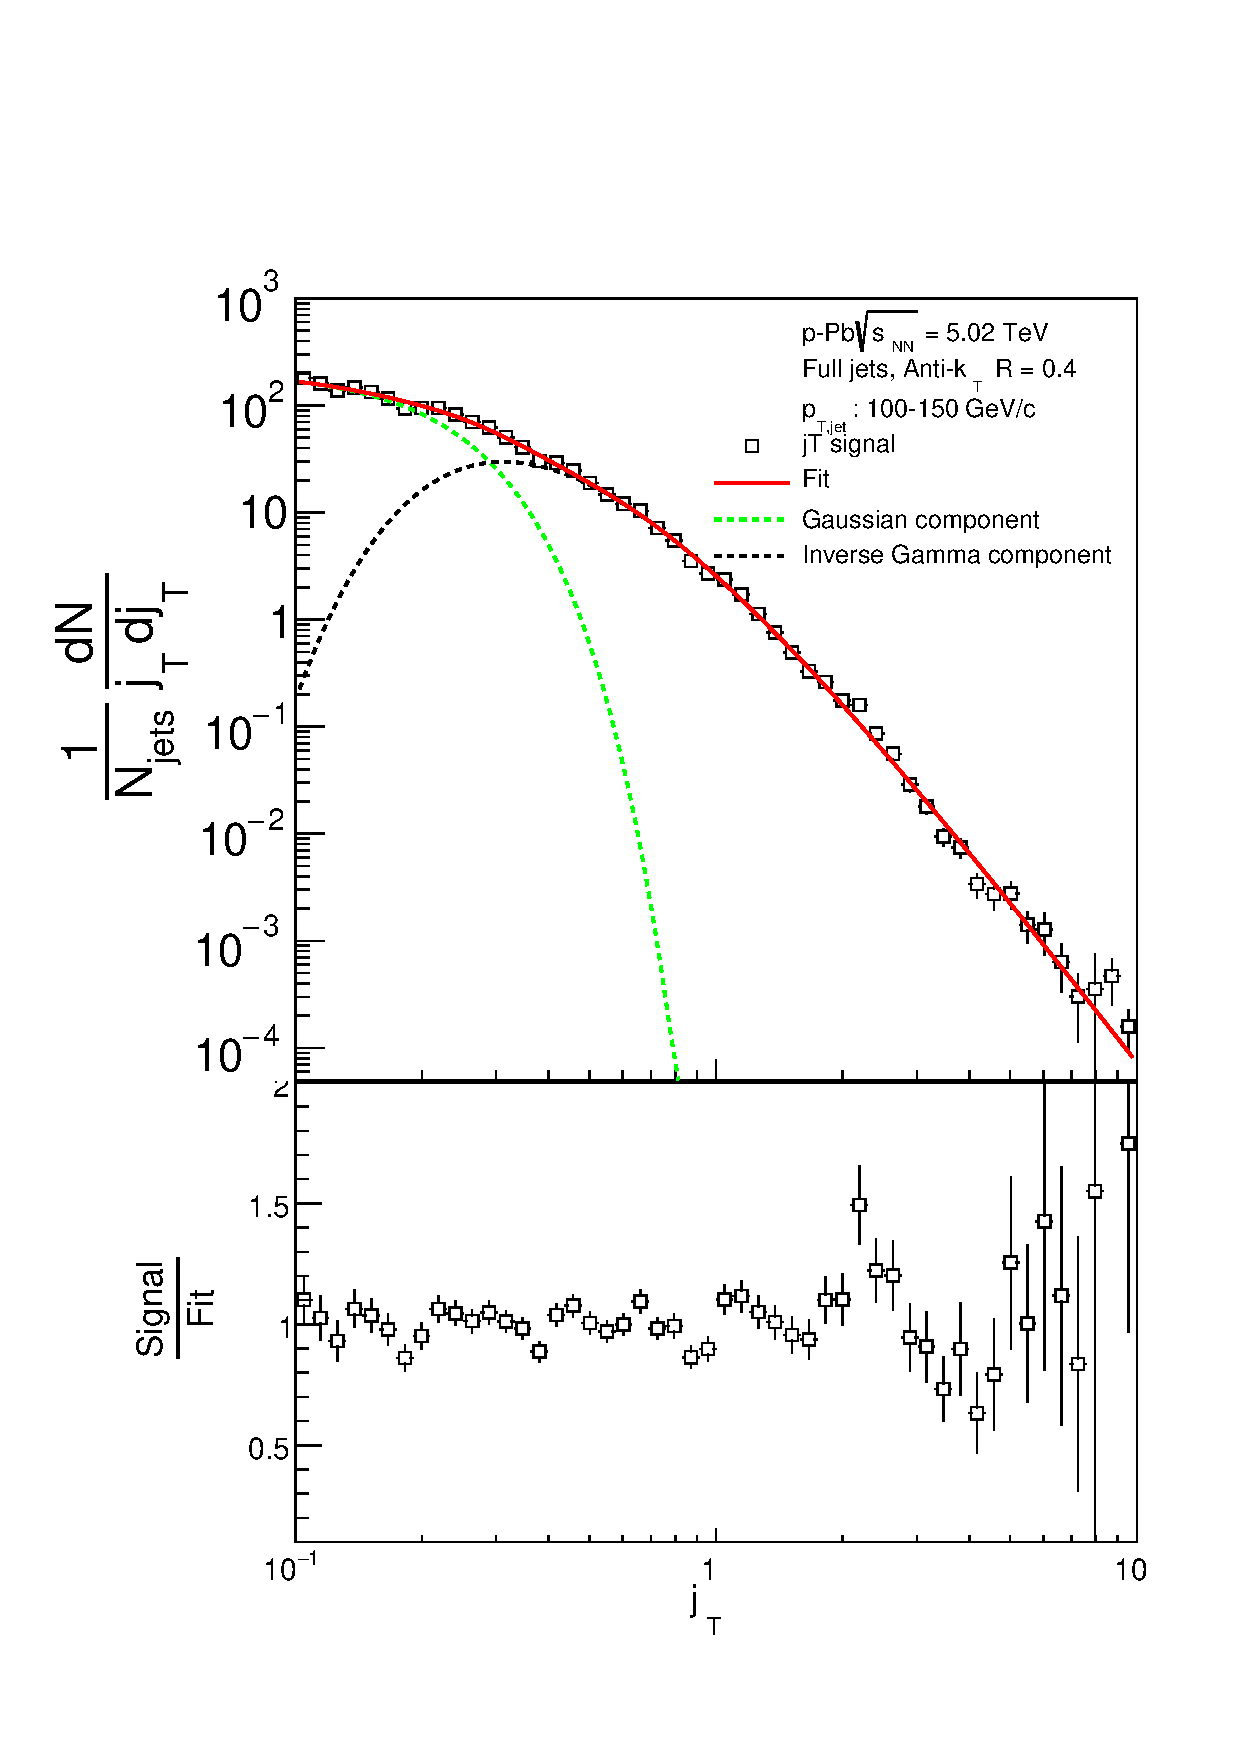
\includegraphics[width=0.95\textwidth]{results/JetConejTSignalFit/JetConejTSignalFitNFin00JetPt07perconeBgBayes}
\end{subfigure}
\caption{$\jt{}$ signal distributions fitted with the two component model in different jet $\pt{}$ bins}
\label{fig:fits}
\end{figure}

To characterise the widening of the $\jt{}$ distribution we can then extract the RMS values of the fits. Resulting RMS values with systematic errors are shown separately for the two components in Fig.~\ref{fig:rmsyield}. Here it is seen that the width of the narrow component shows no or only a weak dependence on the transverse momentum of the jet, $\pt{jet}$. Wide component on the other increases clearly with increasing $\pt{jet}$.

Figure \ref{fig:rms} shows RMS values for both components combined and overlaid with \pythia and Hewig simulations. As seen in the figure all the \pythia models reproduce the data well, both the wide and narrow component. Herwig, on the other hand, seems to produce significantly wider $\jt{}$ distributions. This difference seems to get larger with increasing $\pt{jet}$. For the narrow component Herwig gives a good representation of the data.
\begin{figure}[htb]
\centering
\begin{subfigure}{0.49\textwidth}
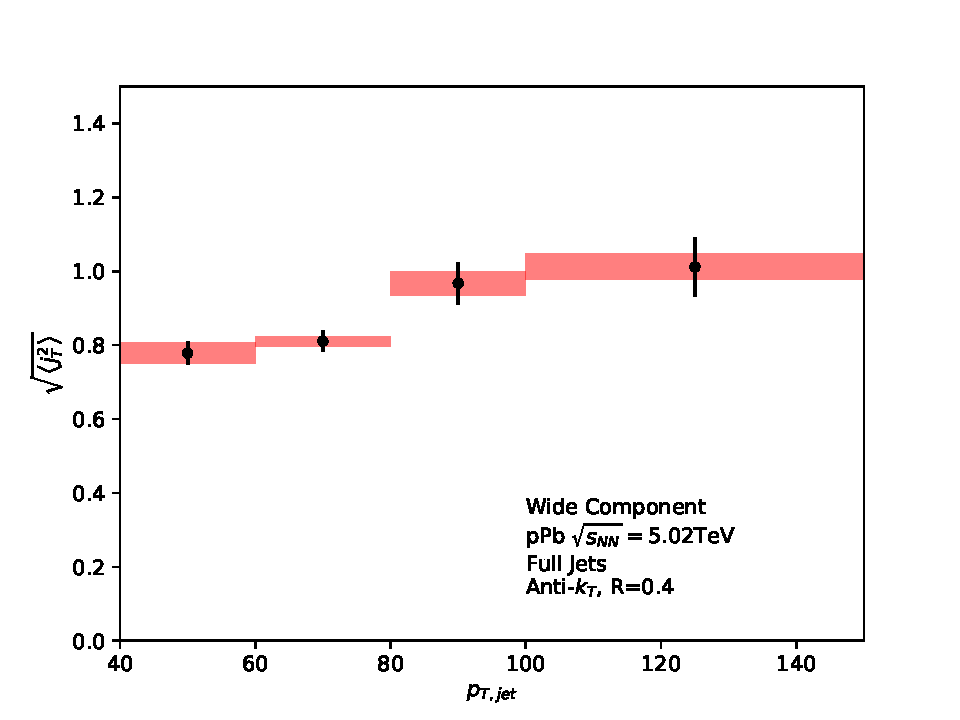
\includegraphics[width=0.95\textwidth]{results/gammaRMSWithSystematics}
\end{subfigure}
%\begin{subfigure}{0.5\textwidth}
%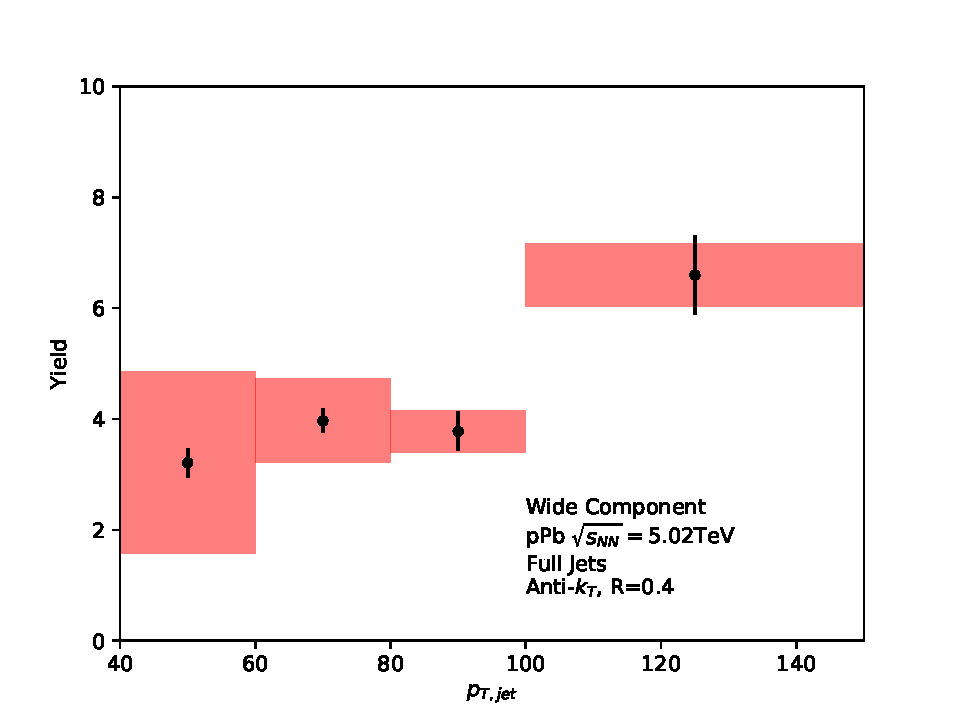
\includegraphics[width=0.95\textwidth]{results/gammaYieldWithSystematics}
%\end{subfigure}
\begin{subfigure}{0.49\textwidth}
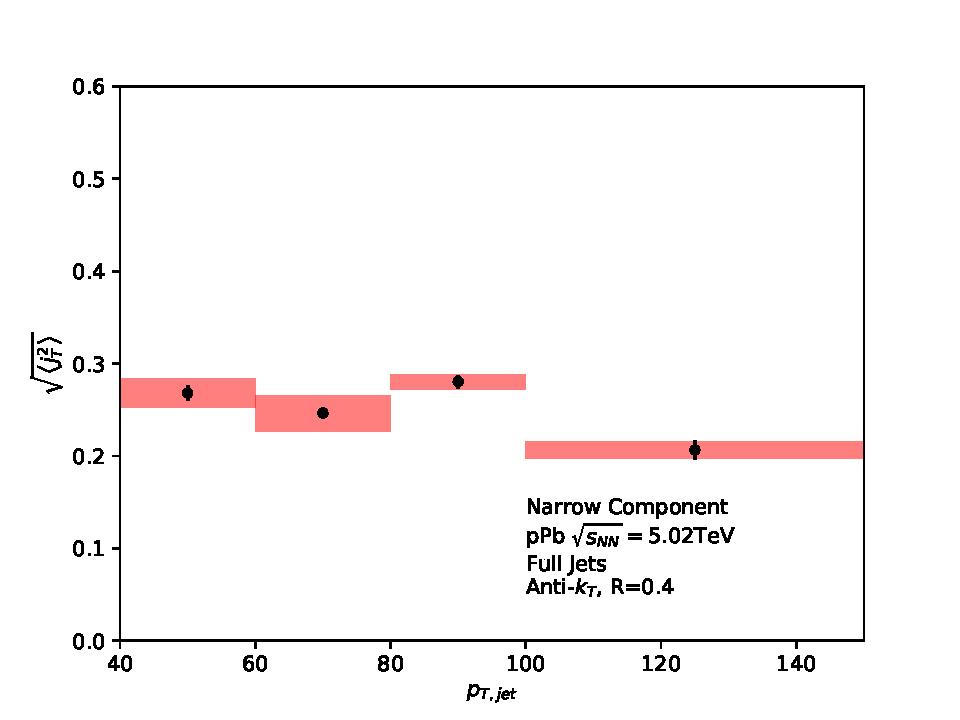
\includegraphics[width=0.95\textwidth]{figures/results/gausRMSWithSystematics}
\end{subfigure}
%\begin{subfigure}{0.5\textwidth}
%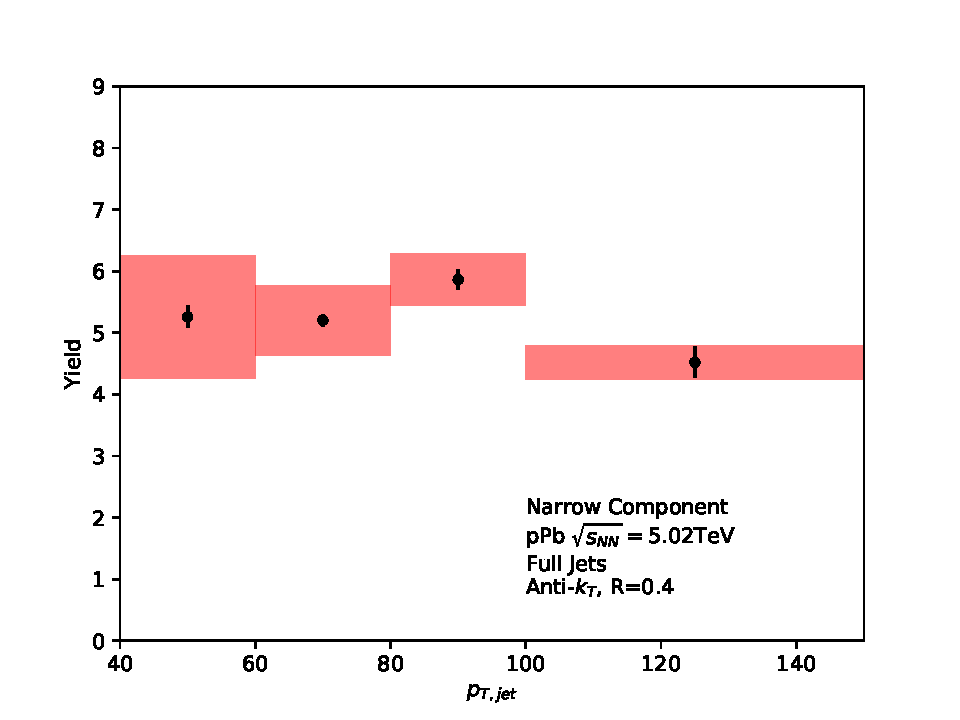
\includegraphics[width=0.95\textwidth]{results/gausYieldWithSystematics}
%\end{subfigure}
\caption{RMS values extracted from the fits for the Gaussian (narrow) and inverse gamma (wide) components}
\label{fig:rmsyield}
\end{figure}

\begin{figure}[htb]
\centering
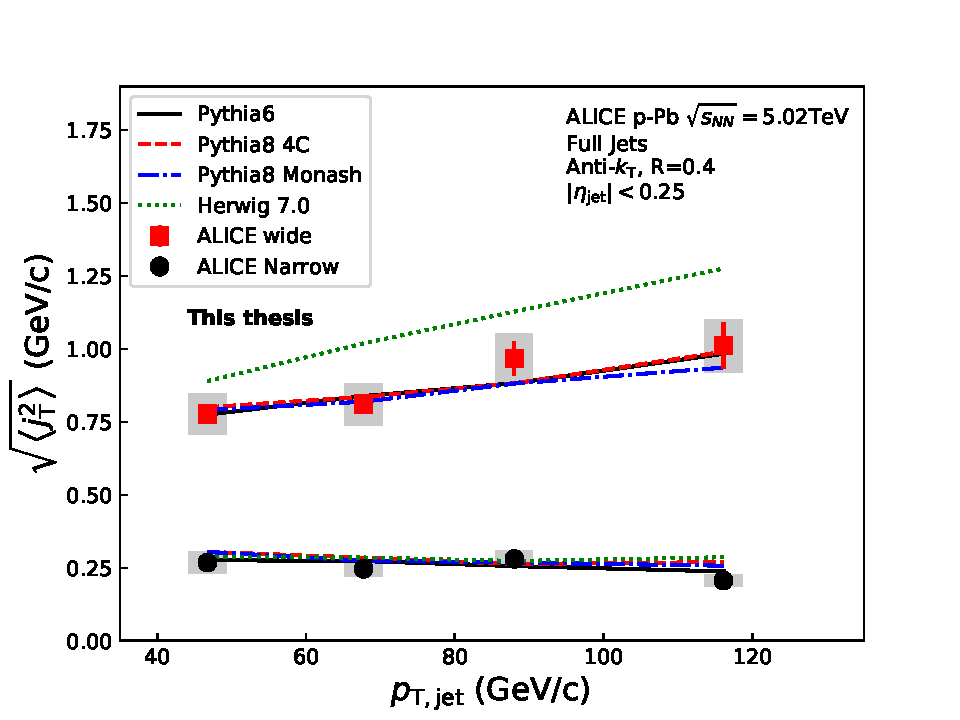
\includegraphics[width=0.65\textwidth]{figures/results/RMSWithSystematics_Pythia}
\caption{RMS values extracted from the fits for the Gaussian (narrow) and inverse gamma (wide) components}
\label{fig:rms}
\end{figure}

\subsection{High multiplicity}
The analysis was repeated taking only events with high multiplicity. Three different multiplicity percentile cuts were used; \unit[10]{\%}, \unit[1]{\%} and \unit[0.1]{\%}. We used ZDC(TODO) as a centrality estimator. As argued in section ~\ref{sec:smallsystemcentrality} the zero-degree energy deposit should provide a centrality estimator with minimal bias from jet production. Resulting $\jt{}$ signal distributions are shown Fig.~\ref{fig:highm}. As the statistics are limited in the high multiplicity runs, it was hard to achieve stable fits to the distributions. Thus the RMS values are not shown. 

From the figure one can observe no systematic modification when tighter multiplicity cuts are introduced. There is a hint of a dip at $\jt{} \approx 2$, but it is well within statistical error bars. This is also the region where the signal is most sensitive to background subtraction. Higher multiplicity events will naturally have higher background. Background estimation is done separately for the multiplicity bins. Thus it is not expected that different backgrounds would cause a difference, but this possibility can't be ruled out.

As described in Sec.~\ref{sec:smallsystem} no conclusive evidence of jet modification in \pPb collisions has been observed.  Most jet observables show no difference between \pp and \pPb collisions. Thus any difference in $\jt{}$ would also be small. 


\begin{figure}[htb]
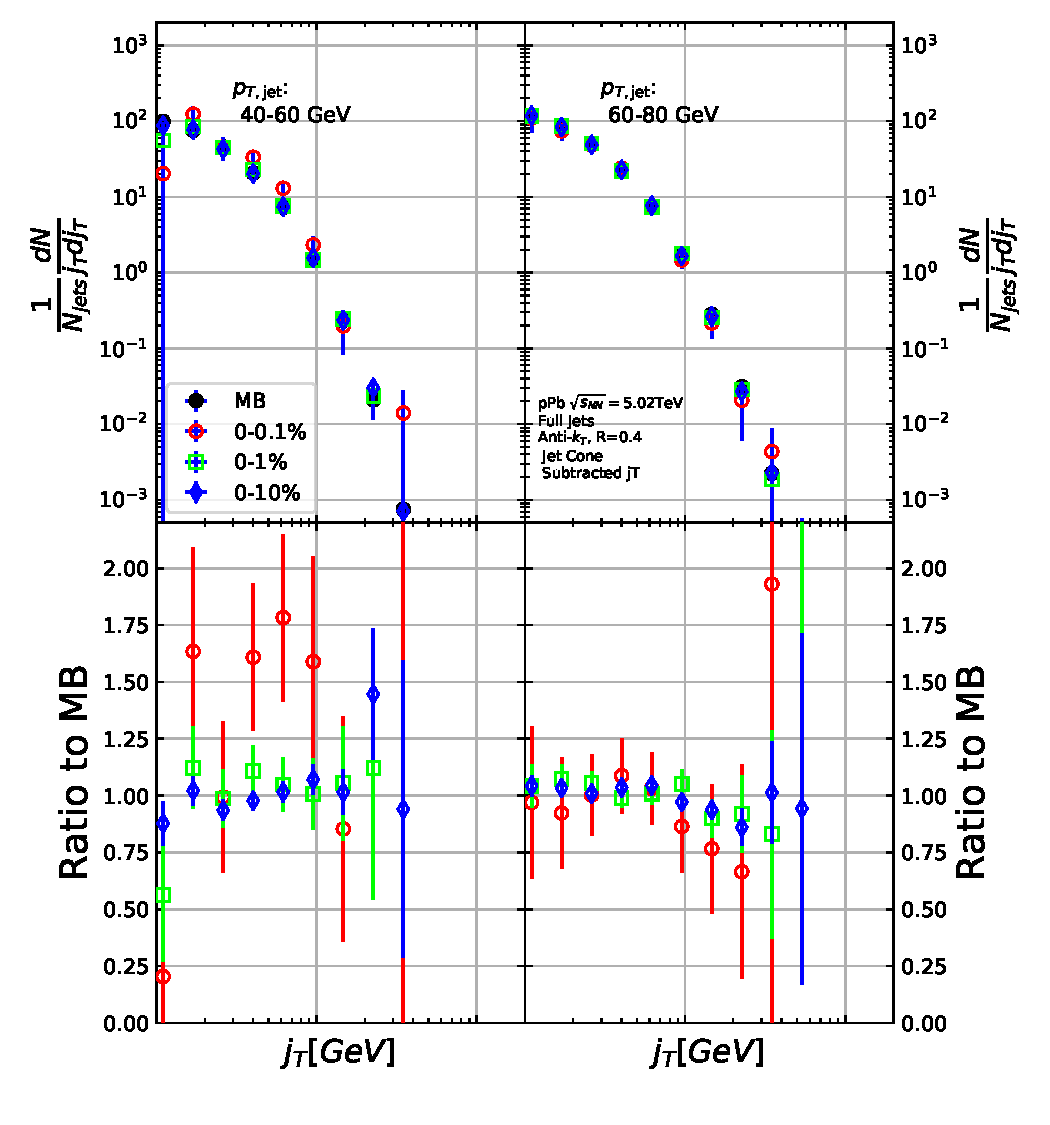
\includegraphics[width=0.95\textwidth]{results/HighMJetConeJtSignalPtFrom3To8.pdf}
\caption{$\jt{}$ distributions for high multiplicity \pPb~ events. {\color{red} Replace figure with ZDC results}}
\label{fig:highm}
\end{figure}



